\documentclass[10pt]{article}

\usepackage[preprint]{tmlr}

\usepackage[utf8]{inputenc}
\usepackage{amsmath,amssymb,amsthm}
\usepackage{mathtools}
\usepackage{hyperref}
\usepackage{cleveref}
\usepackage{booktabs}
\usepackage{multirow}
\usepackage{enumitem}
\usepackage{xcolor}
\usepackage{graphicx}
\usepackage{microtype}
\usepackage{tikz}
\usetikzlibrary{arrows.meta, decorations.pathreplacing, patterns,
                shapes.geometric, positioning, calc, backgrounds, fit}

% colours used by the two figures
\definecolor{triblue}{RGB}{30,100,180}
\definecolor{trigreen}{RGB}{30,140,80}
\definecolor{trired}{RGB}{190,40,40}
\definecolor{trigold}{RGB}{200,150,0}

\newtheorem{theorem}{Theorem}[section]
\newtheorem{lemma}[theorem]{Lemma}
\newtheorem{corollary}[theorem]{Corollary}
\newtheorem{definition}[theorem]{Definition}

\newcommand{\R}{\mathbb{R}}
\newcommand{\conf}{\mathrm{conf}}
\newcommand{\ans}{\mathrm{ans}}

\title{The Hallucination Trilemma: A Topological Impossibility\\
       for Faithful, Covering, and Calibrated Language Models}

\author{\name Manish Bhatt \email manish.bhatt13212@gmail.com \\
      \addr OWASP
      \AND
      \name Ken Huang \email ken@distributedapps.ai \\
      \addr Distributedapps.ai}

\def\month{05}
\def\year{2026}
\def\openreview{\url{https://openreview.net/forum?id=XXXX}}

\begin{document}

\maketitle

\begin{abstract}
We prove that no question-answering model with a continuous confidence map
on a connected question space can be simultaneously \emph{faithful}
(confidence $\geq\tfrac12$ implies a correct answer), \emph{covering} (it
returns both correct and wrong answers), and \emph{strictly calibrated}
(confidence above/below $\tfrac12$ iff correct/wrong). Coverage supplies
witnesses on both sides of the threshold; connectedness and continuity force
a threshold-confidence question through the intermediate value theorem;
calibration pins its truth-distance to zero; faithfulness demands that it be
strictly negative. The contradiction is structural---an application of the
IVT---not a statistical claim about any current system. Crucially, the three
conditions are not an adversarial construction but the ideal that model
builders actively strive for: a model that is trustworthy when confident,
useful across questions, and honest about what it knows. Our result shows this
sought-after ideal is not merely hard to reach but formally unreachable, and
the closer a model is driven toward it---as calibration is idealized toward the
zero-slack biconditional---the tighter the obstruction binds. The same two-line
core fires with no topology once a single boundary question exists, and the
result extends to multi-turn, stochastic, and approximately calibrated
settings, where it becomes quantitative. All results are machine-verified in Lean~4 against
Mathlib v4.28, sorry-free, depending only on the three standard kernel axioms.
\end{abstract}

% ============================================================
\section{Introduction}
\label{sec:intro}

Hallucination---a model producing a confident but wrong answer---is one of
the most reliably observed failures of deployed language models
\citep{maynez2020faithfulness,ji2023survey,zhang2023siren}. The usual fixes
are empirical: more data, RLHF, temperature tuning, post-hoc calibration.
We show that under idealized conditions there is a mathematical obstruction
that no amount of training removes.

Consider any model that returns an answer together with a confidence score.
Three properties are natural to want:
\begin{itemize}[nosep,leftmargin=1.5em]
\item \textbf{Faithful:} when at least half-confident, the answer is correct.
\item \textbf{Covering:} the model is sometimes right and sometimes wrong---it
  does not refuse everything or output a constant.
\item \textbf{Calibrated:} confidence tracks correctness in both
  directions---high confidence means right, low confidence means wrong.
\end{itemize}
For a continuous confidence map on a connected question space these three
cannot coexist. The proof needs no training assumptions, no architecture, no
statistics: it is the intermediate value theorem.

\paragraph{Why.}
Coverage gives a question $q_+$ answered correctly and a question $q_-$
answered wrongly. Calibration turns these into confidence above $\tfrac12$ at
$q_+$ and below $\tfrac12$ at $q_-$. If $Q$ is connected and the confidence
map is continuous, the IVT forces confidence to equal $\tfrac12$ at some
$q_0$. Calibration then pins the answer at $q_0$ exactly on the truth
boundary. But faithfulness says half-confident answers must be strictly
correct. At $q_0$ the model is exactly half-confident and its answer is on the
boundary, not strictly correct---a contradiction.

\paragraph{What it says about real models.}
Coverage holds for every useful model; the binding condition is calibration.
The theorem does \emph{not} claim deployed LLMs meet all three and derive a
contradiction---no current model satisfies strict biconditional calibration.
It says the design target the field is working toward is unreachable, and that
the constraint tightens as calibration improves. \Cref{sec:extensions} makes
this quantitative: under $\varepsilon$-calibration a threshold-confidence
question has truth-distance in $[-\varepsilon,0)$, collapsing to
$0\le\delta_M(q_0)<0$ at $\varepsilon=0$.

\paragraph{Relation to prior work.}
\citet{xu2024hallucination} prove hallucination via computability (finite
capacity cannot cover all computable functions), an argument about the
distribution boundary that ignores calibration.
\citet{karpowicz2025impossibility} derive a conflict among four
mechanism-design conditions via proper scoring rules. Neither uses the IVT or
makes calibration central. Our result differs on all three counts---three
conditions with calibration explicit, an IVT-only proof, and machine
verification---and is, to our knowledge, the first hallucination impossibility
formalized in a proof assistant.

% ============================================================
\section{Setup}
\label{sec:setup}

Let $Q$ be the \emph{question space}, a connected topological space, and $A$
the \emph{answer space}. A \emph{model} is a continuous map
$M\colon Q \to A \times \R$ with components $\ans(q)=(M(q))_1$ and
$\conf(q)=(M(q))_2$. Connectedness is the key hypothesis; the Lean proof uses
only preconnectedness of $Q$ and continuity of the confidence coordinate, not
a path between questions.

Correctness is a continuous signed \emph{truth-distance}
$\delta\colon Q\times A\to\R$: $\delta(q,a)<0$ means $a$ is correct at $q$,
$\delta(q,a)>0$ means wrong, and $\delta(q,a)=0$ is the boundary. Write
$\delta_M(q)=\delta(q,\ans(q))$. This subsumes soft factuality scores,
semantic-similarity thresholds, and any score with a natural zero. The
threshold $\tfrac12$ is conventional; replacing it by any constant $c$ gives
an identical proof.

\begin{definition}[Faithfulness]\label{def:faithful}
$\conf(q)\ge\tfrac12 \Rightarrow \delta_M(q)<0$ for every $q$.
\end{definition}
\begin{definition}[Coverage]\label{def:covering}
There exist $q_+,q_-$ with $\delta_M(q_+)<0$ and $\delta_M(q_-)>0$.
\end{definition}
\begin{definition}[Strict calibration]\label{def:calibrated}
For every $q$: $\;\conf(q)>\tfrac12 \iff \delta_M(q)<0\;$ and
$\;\conf(q)<\tfrac12 \iff \delta_M(q)>0$.
\end{definition}

Strict calibration is a biconditional between the side of the threshold and
the sign of the truth-distance. It differs from statistical calibration (where
$\conf$ approximates the probability of correctness) and is the condition that
gives the argument its bite: it pins $\delta_M$ to zero wherever confidence
crosses $\tfrac12$.

% ============================================================
\section{The Trilemma}
\label{sec:trilemma}

\begin{theorem}[Boundary question]\label{thm:boundary}
Let $Q$ be connected and $M$ continuous with continuous $\delta$. If $M$ is
covering and strictly calibrated, there is $q_0\in Q$ with $\conf(q_0)=\tfrac12$
and $\delta_M(q_0)=0$.
\end{theorem}
\begin{proof}
Coverage and calibration give $\conf(q_+)>\tfrac12$ and $\conf(q_-)<\tfrac12$.
The confidence map is continuous on the connected $Q$, so by the IVT it equals
$\tfrac12$ at some $q_0$. There it is neither above nor below the threshold, so
both biconditionals fire negatively: $\delta_M(q_0)$ is neither $<0$ nor $>0$,
hence $=0$.
\end{proof}

\begin{theorem}[Hallucination Trilemma]\label{thm:trilemma}
No continuous model on a connected question space is simultaneously faithful,
covering, and strictly calibrated.
\end{theorem}
\begin{proof}
\Cref{thm:boundary} gives $q_0$ with $\conf(q_0)=\tfrac12$ and
$\delta_M(q_0)=0$. Since $\conf(q_0)\ge\tfrac12$, faithfulness requires
$\delta_M(q_0)<0$, contradicting $\delta_M(q_0)=0$.
\end{proof}

The proof uses nothing about architecture, training, or parameter count---only
continuity of $M$ and connectedness of $Q$. Any model satisfying the three
conditions must violate one of these two.

\paragraph{Tightness.}
\label{par:tightness}
The threshold is exact: relaxing faithfulness by any $\varepsilon>0$ breaks the
impossibility. On $Q=[0,1]$ with $\conf(q)=1-q$ and $\delta_M(q)=q-\tfrac12$,
strict calibration and coverage hold, and
$(\tfrac12+\varepsilon)$-faithfulness holds for every $\varepsilon>0$; only
standard faithfulness fails, at $q=\tfrac12$. The band
$[\tfrac12,\tfrac12+\varepsilon)$ is the price of escape.

\paragraph{Each hypothesis is necessary.}
\label{sec:counterexamples}
Dropping any single condition lets the other two coexist (the dashed edges of
\Cref{fig:trilemma}, left).
\emph{Not faithful:} the tightness model above---calibrated and covering, but
$\delta_M=0$ at $\conf=\tfrac12$.
\emph{Not covering:} constant $\conf=\tfrac34$ with $\delta_M<0$ everywhere is
faithful and calibrated, but has no wrong-answer witness.
\emph{Not continuous:} $\conf=\tfrac34$ on $(\tfrac12,1]$ and $\tfrac14$ on
$[0,\tfrac12)$ with matching signs is faithful, covering, and calibrated
pointwise, but jumps at $\tfrac12$.

\begin{figure}[t]
\centering
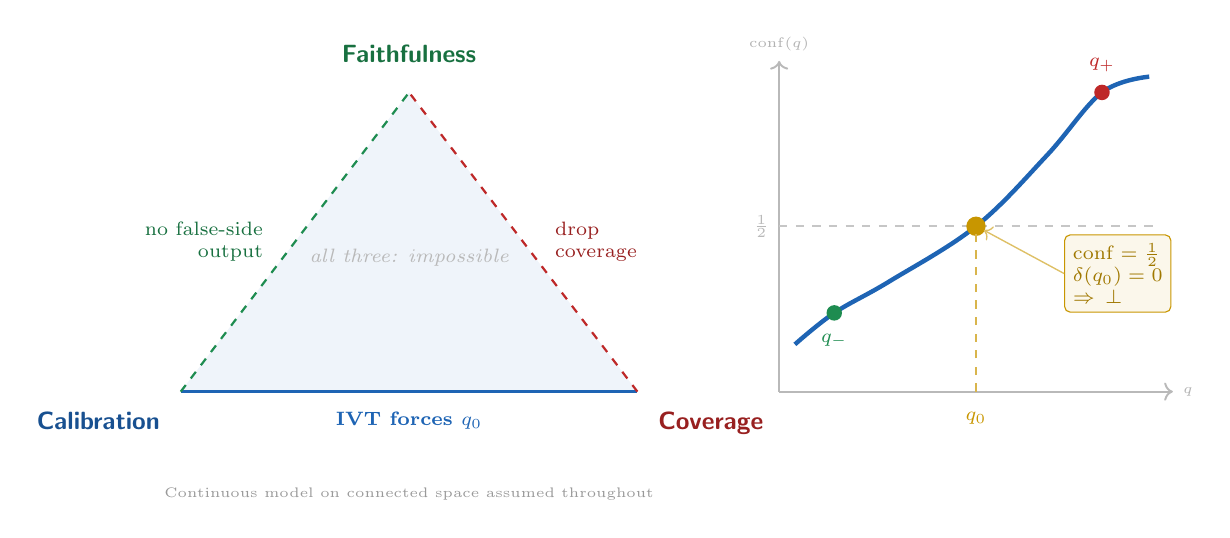
\begin{tikzpicture}[x=1cm, y=1cm]

%% LEFT PANEL – the trilemma triangle
\coordinate (TF) at (3.1, 3.8);   % Faithfulness – top
\coordinate (TC) at (0.2, 0);     % Calibration  – bottom-left
\coordinate (TV) at (6.0, 0);     % Coverage     – bottom-right
\fill[triblue!7] (TF) -- (TC) -- (TV) -- cycle;
\draw[triblue,  very thick]              (TC) -- (TV);
\draw[trigreen, thick, dashed]           (TC) -- (TF);
\draw[trired,   thick, dashed]           (TV) -- (TF);
\node[above, font=\small\bfseries\sffamily, text=trigreen!80!black]
  at (3.1, 4.05) {Faithfulness};
\node[below left, font=\small\bfseries\sffamily, text=triblue!80!black,
      xshift=-4pt, yshift=-4pt] at (TC) {Calibration};
\node[below right, font=\small\bfseries\sffamily, text=trired!80!black,
      xshift=4pt, yshift=-4pt] at (TV) {Coverage};
\node[below, yshift=-4pt, font=\scriptsize, text=triblue, align=center]
  at (3.1, 0) {\textbf{IVT forces $q_0$}};
\node[left, xshift=-8pt, font=\scriptsize, text=trigreen!80!black, align=right]
  at (1.65, 1.9) {no false-side\\output};
\node[right, xshift=8pt, font=\scriptsize, text=trired!80!black, align=left]
  at (4.55, 1.9) {drop\\coverage};
\node[font=\scriptsize\itshape, text=gray!55]
  at (3.1, 1.7) {all three: impossible};
\node[font=\tiny, text=black!40, align=center]
  at (3.1, -1.3) {Continuous model on connected space assumed throughout};

%% RIGHT PANEL – the IVT crossing
\begin{scope}[shift={(7.8, 0)}]
  \draw[->, gray!55, line width=0.7pt] (0, 0) -- (5.0, 0)
    node[right, font=\tiny, text=gray!60] {$q$};
  \draw[->, gray!55, line width=0.7pt] (0, 0) -- (0, 4.2)
    node[above, font=\tiny, text=gray!60] {$\mathrm{conf}(q)$};
  \draw[gray!45, dashed, line width=0.6pt] (0, 2.1) -- (4.8, 2.1);
  \node[left, font=\tiny, text=gray!55] at (0, 2.1) {$\tfrac{1}{2}$};
  \draw[triblue, line width=1.6pt] plot[smooth, tension=0.6] coordinates
    {(0.2,0.6) (0.7,1.0) (1.4,1.4) (2.5,2.1) (3.4,3.0) (4.1,3.8) (4.7,4.0)};
  \fill[trigreen] (0.7, 1.0) circle (2.8pt);
  \node[below, yshift=-4pt, font=\scriptsize, text=trigreen] at (0.7, 1.0) {$q_-$};
  \fill[trired] (4.1, 3.8) circle (2.8pt);
  \node[above, yshift=4pt, font=\scriptsize, text=trired] at (4.1, 3.8) {$q_+$};
  \fill[trigold] (2.5, 2.1) circle (3.5pt);
  \draw[trigold!70, dashed, line width=0.7pt] (2.5, 0) -- (2.5, 2.1);
  \node[below, yshift=-4pt, font=\scriptsize\bfseries, text=trigold]
    at (2.5, 0) {$q_0$};
  \node[draw=trigold, fill=trigold!8, rounded corners=2pt,
        font=\scriptsize, text=trigold!80!black, align=left,
        inner sep=3pt] (callout)
    at (4.3, 1.5) {$\mathrm{conf}=\tfrac{1}{2}$\\$\delta(q_0)=0$\\$\Rightarrow\,\bot$};
  \draw[->, trigold!60, line width=0.5pt] (callout.west) -- (2.6, 2.05);
\end{scope}
\end{tikzpicture}
\vspace{2pt}
\caption{\textbf{Left:} the trilemma. No continuous model on a connected space
satisfies all three; the solid edge is the main result, the dashed edges the
counterexamples. \textbf{Right:} the IVT argument. Coverage gives $q_-$
($\conf<\tfrac12$) and $q_+$ ($\conf>\tfrac12$); connectedness forces the
crossing $q_0$; calibration pins $\delta(q_0)=0$; faithfulness then demands
$\delta(q_0)<0$---contradiction.}
\label{fig:trilemma}
\end{figure}

% ============================================================
\section{Extensions}
\label{sec:extensions}

\paragraph{Discrete core.}
The IVT is used only to \emph{produce} the boundary question; the contradiction
itself needs no topology.

\begin{theorem}[Discrete impossibility]\label{thm:pure-discrete}
Let $Q,A$ be arbitrary sets with no topology. No model can be faithful,
strictly calibrated, and have a question $q^*$ with $\delta_M(q^*)=0$.
\end{theorem}

Indeed, $\delta_M(q^*)=0$ makes both calibration biconditionals fail unless
$\conf(q^*)=\tfrac12$, and faithfulness then demands $\delta_M(q^*)<0$. The
continuous trilemma factors through this: IVT supplies $q^*$ from two-sided
coverage and connectedness (\Cref{fig:extensions}b). On a genuinely
disconnected set with no boundary question, all three conditions can hold---a
real escape---so the discrete version assumes a boundary question
(``three-sided coverage''). Equivalently: under strict calibration, a model is
faithful iff it has \emph{no} boundary questions.

\paragraph{Stochastic models.}
Randomizing at $q_0$ does not help. Let $\bar c,\bar\delta$ be expected
confidence and truth-distance; if they are continuous and meet the three
conditions in expectation, the trilemma yields $q_0$ with $\bar\delta(q_0)=0$.
The sample-level version is sharper.

\begin{theorem}[Stochastic dichotomy]\label{thm:dichotomy}
Let $c,d\colon\Omega\to\R$ be measurable on a probability space $(\Omega,\mu)$
with $d$ integrable, $\int d\,d\mu=0$, sample faithfulness
($c\ge\tfrac12\Rightarrow d<0$) $\mu$-a.e., and $\mu\{c\ge\tfrac12\}>0$. Then
$\mu\{d>0\}>0$.
\end{theorem}
\begin{proof}
If $\mu\{d>0\}=0$ then $-d\ge0$ a.e.\ with $\int(-d)\,d\mu=0$, so $d=0$ a.e.
But on $\{c\ge\tfrac12\}$ (positive probability) faithfulness gives $d<0$
a.e.---a contradiction.
\end{proof}

So a stochastic model that is confident with positive probability at $q_0$
hallucinates there with positive probability (\Cref{fig:extensions}a).

\begin{figure}[t]
\centering
\tikzset{
  fbox/.style={draw=#1, fill=#1!9, rounded corners=3pt,
               font=\scriptsize\sffamily, align=center,
               inner sep=5pt, minimum width=2.6cm, minimum height=0.75cm},
  farr/.style={-{Stealth[length=5pt,width=4pt]}, line width=1pt, #1},
}
\begin{tikzpicture}[x=1cm, y=1cm]

%% LEFT PANEL – stochastic dichotomy
\node[font=\small\bfseries\sffamily, anchor=north] at (2.75, 4.5)
  {(a) Stochastic dichotomy at $q_0$};
\draw[->, gray!50, line width=0.7pt] (-0.2, 0) -- (5.3, 0)
  node[right, font=\tiny, text=gray!55] {$\delta$};
\draw[gray!40, dashed, line width=0.7pt] (2.65, -0.4) -- (2.65, 3.6);
\node[below, font=\tiny, text=gray!50] at (2.65, -0.4) {$0$};
\node[font=\scriptsize, text=triblue!80!black, align=center]
  at (1.35, 3.8) {\textit{boundary determinism}\\[1pt]$\delta\leq 0$ a.s.};
\node[font=\scriptsize, text=trired!80!black, align=center]
  at (4.0, 3.8) {\textit{hallucination}\\[1pt]$\mu\{\delta>0\}>0$};
\begin{scope}[opacity=0.5]
  \fill[triblue!55] plot[smooth, tension=0.7] coordinates
    {(0.1,0)(0.4,0.3)(0.8,1.2)(1.3,2.6)(1.7,2.8)(2.1,1.8)(2.5,0.5)(2.65,0)}
    -- (2.65,0) -- (0.1,0) -- cycle;
  \draw[triblue, line width=1.1pt] plot[smooth, tension=0.7] coordinates
    {(0.1,0)(0.4,0.3)(0.8,1.2)(1.3,2.6)(1.7,2.8)(2.1,1.8)(2.5,0.5)(2.65,0)};
\end{scope}
\begin{scope}[opacity=0.5]
  \fill[trired!50] plot[smooth, tension=0.7] coordinates
    {(2.65,0)(2.8,0.4)(3.1,1.4)(3.6,2.5)(4.0,2.7)(4.4,1.6)(4.8,0.5)(5.1,0)}
    -- (5.1,0) -- (2.65,0) -- cycle;
  \draw[trired, line width=1.1pt] plot[smooth, tension=0.7] coordinates
    {(2.65,0)(2.8,0.4)(3.1,1.4)(3.6,2.5)(4.0,2.7)(4.4,1.6)(4.8,0.5)(5.1,0)};
\end{scope}
\draw[trigold, line width=1.2pt] (2.65, -0.15) -- (2.65, 0.0);
\fill[trigold] (2.65, -0.25) -- (2.35,-0.5) -- (2.95,-0.5) -- cycle;
\node[below, yshift=-2pt, font=\tiny, text=trigold!80!black]
  at (2.65, -0.5) {$\mathbb{E}[\delta]=0$};
\draw[->, triblue!60, line width=0.5pt, shorten >=3pt] (1.35, 3.55) -- (1.55, 3.05);
\draw[->, trired!60, line width=0.5pt, shorten >=3pt] (4.0, 3.55) -- (3.85, 3.0);

%% RIGHT PANEL – continuous vs discrete
\begin{scope}[shift={(6.8, 0)}]
\node[font=\small\bfseries\sffamily, anchor=north] at (3.1, 4.5)
  {(b) Continuous vs.\ discrete};
\node[fbox=triblue] (cov)  at (1.3, 3.2) {Two-sided coverage\\+ connectedness};
\node[fbox=triblue] (wit)  at (1.3, 1.9) {$\exists\,q_0$ with $\delta(q_0)=0$};
\draw[farr=triblue] (cov) -- (wit)
  node[midway, left=4pt, font=\tiny, text=triblue!80!black] {IVT};
\node[fbox=trigreen] (thr) at (1.3, 0.6) {Three-sided coverage};
\draw[farr=trigreen, dashed] (thr.north) -- (wit.south)
  node[midway, left=4pt, font=\tiny, text=trigreen!80!black] {direct};
\node[font=\tiny\itshape, text=triblue!70!black, anchor=east]
  at (0.05, 2.55) {continuous};
\node[font=\tiny\itshape, text=trigreen!70!black, anchor=east]
  at (0.05, 0.6) {discrete};
\node[fbox=trired] (core) at (4.4, 1.9)
  {Faithful\\+ Calibrated\\+ $\delta(q_0)=0$\\$\Rightarrow\;\bot$};
\draw[farr=gray!60] (wit.east)  -- (core.west);
\draw[farr=gray!60] (thr.east) to[out=0, in=270] (core.south);
\node[font=\tiny\itshape, text=gray!55, anchor=south] at (4.4, 2.85) {shared core};
\end{scope}
\end{tikzpicture}
\vspace{2pt}
\caption{\textbf{(a)} At the forced point $q_0$ where $\mathbb{E}[\delta]=0$, a
confident stochastic model faces a dichotomy: all mass at $\delta=0$ (boundary
determinism) or positive mass at $\delta>0$ (hallucination). \textbf{(b)} The
continuous and discrete trilemmas share a two-line core (right), differing only
in how the witness $q_0$ is produced---IVT from two-sided coverage vs.\ explicit
three-sided coverage.}
\label{fig:extensions}
\end{figure}

\paragraph{Multi-turn and antipodal.}
A finite product of connected spaces is connected, so the history space $Q^T$
is connected and \Cref{thm:trilemma} applies to history-dependent
$M\colon Q^T\to A\times\R$ unchanged: context does not remove the obstruction.
When questions come in opposite pairs via a continuous involution
$\sigma$ with $\delta_M(\sigma(q))=-\delta_M(q)$, the IVT forces a zero with no
coverage hypothesis at all---coverage becomes automatic.

\paragraph{Approximate calibration.}
Real models are not strictly calibrated. Call $M$
\emph{$\varepsilon$-calibrated} if $\delta_M(q)<-\varepsilon\Rightarrow
\conf(q)>c+\varepsilon$ and $\delta_M(q)>\varepsilon\Rightarrow\conf(q)<c-\varepsilon$.

\begin{theorem}[Approximate trilemma]\label{thm:approx}
Let $\varepsilon\ge0$, $Q$ connected, $\conf$ continuous. If $M$ has
$\varepsilon$-coverage, is two-sided $\varepsilon$-calibrated, and is
$c$-faithful, then some $q_0$ has $\conf(q_0)=c$ and
$\delta_M(q_0)\in[-\varepsilon,0)$.
\end{theorem}
\begin{proof}
$\varepsilon$-calibration sends the coverage witnesses to $\conf>c$ and
$\conf<c$, so IVT gives $\conf(q_0)=c$. Faithfulness gives $\delta_M(q_0)<0$;
and $\delta_M(q_0)<-\varepsilon$ would force $\conf(q_0)>c+\varepsilon$, so
$\delta_M(q_0)\ge-\varepsilon$.
\end{proof}

At $\varepsilon=0$ the conclusion is $0\le\delta_M(q_0)<0$---the exact
contradiction. Improving calibration shrinks the margin: calibration and
faithfulness are not independent. Taking $Q_{\mathrm{in}}$ correct and
$Q_{\mathrm{ood}}$ wrong as the two witnesses, $q_0$ lies in neither, i.e.\ in
the in-distribution/OOD transition band---the impossibility localizes there.

% ============================================================
\section{Formalization, Related Work, and Conclusion}
\label{sec:lean}

\paragraph{Lean.}
All results are machine-verified in Lean~4 against Mathlib v4.28, with no
\texttt{sorry} and every headline theorem reducing to
$\{\texttt{propext},\allowbreak \texttt{Quot.sound},\allowbreak
\texttt{Classical.choice}\}$. The core (\texttt{HoF\_07}) applies
\texttt{IsPreconnected.intermediate\_value2} for the IVT step and two
\texttt{linarith} calls for the calibration squeeze; the discrete, stochastic,
and approximate results appear in \texttt{HoF\_10}--\texttt{12}
(\texttt{integral\_eq\_zero\_iff\_of\_nonneg\_ae} for
\Cref{thm:dichotomy}, \texttt{approx\_trilemma} and
\texttt{exact\_from\_approx} for \Cref{thm:approx}). Sources are in the
submission.

\begin{table}[h]
\centering
\small
\renewcommand{\arraystretch}{1.2}
\caption{Comparison with prior hallucination impossibility results.}
\label{tab:comparison}
\begin{tabular}{lccc}
\toprule
& \citet{xu2024hallucination} & \citet{karpowicz2025impossibility} & \textbf{This work} \\
\midrule
Proof technique & Computability & Mech.\ design + scoring & Topology (IVT) \\
Architecture-independent & \checkmark & \checkmark & \checkmark \\
Addresses calibration & \texttimes & \texttimes & \checkmark \\
Number of conditions & N/A & 4 & 3 \\
Machine-verified & \texttimes & \texttimes & \checkmark \\
\bottomrule
\end{tabular}
\end{table}

\paragraph{Related work.}
Empirical studies measure and taxonomize hallucination
\citep{maynez2020faithfulness,ji2023survey,zhang2023siren} without asking
whether it is structurally unavoidable; the two prior impossibility results
\citep{xu2024hallucination,karpowicz2025impossibility} (\Cref{tab:comparison})
make calibration incidental rather than central. The calibration literature
\citep{guo2017calibration,platt1999probabilistic,zadrozny2002obtaining} treats
miscalibration as correctable---the trilemma says correction costs one of the
other two properties---while selective prediction
\citep{kamath2020selective,feng2020language} is exactly dropping coverage. The
companion Defense Trilemma \citep{anonymous2025defense} applies the same IVT
engine to prompt-injection defenses; Lean has verified substantial mathematics
before \citep{avigad2023mathematics,buzzard2020formalising}, but this is the
first such verification of a hallucination impossibility.

\paragraph{Conclusion.}
No continuous model on a connected question space is simultaneously faithful,
covering, and strictly calibrated, by the intermediate value theorem alone.
Context does not help while the history space stays connected, randomization
gives positive-probability wrong answers, and discrete token space escapes only
until a boundary question appears. The three conditions name the three
available relaxations---abstain, tolerate a threshold band, or accept a weaker
confidence signal---and at least one must give; which is cheapest depends on
how often a deployment operates near its confidence boundary, an empirical
quantity the theorem does not fix.

{\small
\setlength{\bibsep}{3.5pt plus 0.3ex}
\bibliographystyle{tmlr}
\bibliography{hallucination_trilemma_refs}
}

\end{document}
